\documentclass[11pt]{article}
\usepackage[a4paper,margin=2.6cm]{geometry}
\usepackage[T1]{fontenc}
\usepackage{lmodern}
\usepackage{microtype}
\usepackage{amsmath,amssymb}
\usepackage{booktabs}
\usepackage[section]{placeins}
\usepackage{pgfplots}
\pgfplotsset{compat=1.18}
\usepackage[round,authoryear]{natbib}
\usepackage{xurl}
\usepackage[hidelinks]{hyperref}
\usepackage{caption}
\captionsetup{font=small,labelfont=bf}

\newcommand{\NGames}{1{,}510{,}378}
\newcommand{\NTestGames}{1{,}390{,}547}
\newcommand{\NPlayers}{82{,}111}
\newcommand{\NEvents}{14{,}337}
\newcommand{\NSeasons}{11}
\newcommand{\MedianRating}{2229}
\newcommand{\PTenRating}{1842}
\newcommand{\PNinetyRating}{2496}
\newcommand{\DrawRate}{33.4\%}
\newcommand{\WhiteScore}{54.1\%}
\newcommand{\GapScaleLatest}{0.82}
\newcommand{\GapScaleMin}{0.71}
\newcommand{\GapScaleMax}{0.87}
\newcommand{\GapScaleMean}{0.80}
\newcommand{\GapWidePct}{20\%}
\newcommand{\DivisorMean}{500}
\newcommand{\DivisorMin}{460}
\newcommand{\DivisorMax}{570}
\newcommand{\FideAtTwoHundred}{78.3\%}
\newcommand{\ActualAtTwoHundred}{73.9\%}
\newcommand{\FideAtFourHundred}{90.9\%}
\newcommand{\ActualAtFourHundred}{92.2\%}
\newcommand{\AgeTwelve}{$+51$}
\newcommand{\AgeEighteen}{$+32$}
\newcommand{\AgeFifty}{$-36$}
\newcommand{\AgeSixtyFive}{$-71$}
\newcommand{\AgeTwelvePeak}{$+110$}
\newcommand{\WhiteElo}{34}
\newcommand{\WhiteMin}{32}
\newcommand{\WhiteMax}{35}
\newcommand{\FormTenth}{32}
\newcommand{\BrierFide}{0.12383}
\newcommand{\BrierFull}{0.11895}
\newcommand{\WFGain}{3.9\%}
\newcommand{\SimGain}{1.7\%}
\newcommand{\SimTableGain}{1.4\%}
\newcommand{\SimBestSeasons}{11}
\newcommand{\ReturnsAdjusted}{29{,}446}
\newcommand{\GlickoWins}{5}
\newcommand{\UncGrowth}{10}
\newcommand{\DecayMidOneTwo}{$-42$}
\newcommand{\DecayMidTwoFour}{$-50$}
\newcommand{\DecayMidFour}{$-90$}
\newcommand{\DecayOldOneTwo}{$-92$}
\newcommand{\DecayOldTwoFour}{$-111$}
\newcommand{\DecayOldFour}{$-174$}
\newcommand{\DecayYoungOneTwo}{$+39$}
\newcommand{\DecayMidFourCtrl}{$-71$}
\newcommand{\DecayOldFourCtrl}{$-120$}
\newcommand{\DecayYoungOneTwoCtrl}{$+15$}
\newcommand{\NoPandemicFull}{$-$0.0128}
\newcommand{\NoPandemicSim}{$-$0.0063}
\newcommand{\GapBandLow}{0.64}
\newcommand{\GapBandTop}{0.95}
\newcommand{\FullLogLoss}{$-$0.0131}
\newcommand{\SimLogLoss}{$-$0.0065}


\newcommand{\clip}{\operatorname{clip}}
% \input is not expandable in tables; the primitive is
\makeatletter\newcommand{\tabinput}[1]{\@@input #1 }\makeatother

\title{Where FIDE Ratings Miss: A Twelve-Season Out-of-Sample Test of the FIDE Rating System and Proposed Rule Changes}
\author{Nipun Anand\\ Masters' Union, Gurugram, India\\ \texttt{nipun.anand\_ugtbm2030@mastersunion.org}}
\date{September 2026}

\begin{document}
\maketitle

\begin{abstract}
The FIDE rating list is used to seed tournaments, award titles and select players, and every rating on it implies a prediction about game results. This paper tests those predictions on \NGames{} rated classical games played between October 2014 and September 2026, drawn from The Week in Chess and checked against FIDE's own monthly rating lists so that rapid, blitz and Chess960 events are excluded. Corrections are fitted on one season and tested on the next, eleven times. Four systematic errors appear in every test season: the expected-score table overstates rating differences, by about \GapWidePct{} on average and most among lower-rated players; juniors are underrated and older players overrated; adults returning from a break of a year or more are overrated, by amounts that grow with age and length of break, while returning juniors are underrated; and recent overperformance predicts future results. Combined, the corrections reduce the Brier score of the published ratings by \WFGain{}. Proposed rule changes are then replayed month by month against FIDE's current rules, using the K-factor FIDE applied to each player. A wider expectancy table and a one-time, age-dependent adjustment for returning players beat the current rules in all eleven test seasons, reducing the Brier score by \SimGain{}. A higher K-factor for juniors and an uncertainty-based K-factor were worse in every season.
\end{abstract}

\noindent\textbf{Keywords:} chess, Elo rating, paired comparisons, rating systems, forecasting, sports analytics

\section{Introduction}

The International Chess Federation (FIDE) publishes a standard rating for every rated classical player each month. The system descends from \citet{elo1978}: each rating difference maps to an expected score, and after each rating period a player's rating moves by a K-factor times the difference between actual and expected score. The ratings matter well beyond prediction. They decide title norms, tournament seeding, qualification for the Candidates Tournament and invitations to closed events.

Because every rating implies a forecast, the list can be tested directly: if ratings are accurate, expected scores should match actual scores on average, for every group of players. Earlier work has shown that other models forecast chess results better than Elo \citep{sonas2002,glickman1999,sismanis2010,dangauthier2008,coulom2008}. Less attention has gone to two practical questions. Where exactly does the published FIDE list go wrong, and do simple changes to FIDE's own rules fix those errors when the rules are replayed as FIDE would run them?

This paper answers both questions on twelve seasons of data. Its contributions are:
\begin{enumerate}
  \item A cleaned dataset of \NGames{} classical games linked to FIDE IDs, published ratings, birth years and monthly activity, with rapid, blitz and Chess960 events removed by checking each event against FIDE's own game counts.
  \item A walk-forward evaluation over eleven test seasons that identifies four systematic errors in the published ratings and measures how much each correction improves forecasts.
  \item A direct measurement of how much players returning from inactivity are misrated, broken down by age and length of break.
  \item A month-by-month replay of proposed rule changes against FIDE's current rules, using the K-factors FIDE actually applied, which identifies two changes that help in every season and two that do not.
\end{enumerate}

\section{Background}

\subsection{The FIDE rating system}

Under the regulations in force since March 2024 \citep{fide2024}, a player's expected score against an opponent is
\begin{equation}
E_{\mathrm{FIDE}}(D) = \frac{1}{1 + 10^{-\clip(D,\,\pm 400)/400}},
\label{eq:fide}
\end{equation}
where $D$ is the rating difference. Differences beyond 400 points are counted as 400; since October 2025 this applies only to players rated below 2650. After each monthly rating period a player's rating changes by $K \sum (s - E)$ over their rated games. $K$ is 40 for new players until 30 games, and for players until the end of the year of their 18th birthday while rated below 2300; 20 for other players below 2400; and 10 once a player has reached 2400. A player is considered inactive after a year without rated games. Inactive players are left off ranking lists, but their ratings do not change.

In March 2024 FIDE applied a one-time increase to ratings below 2000 to correct compression at the lower end of the list, following a proposal by Jeff Sonas \citep{sonasfide}.

\subsection{Related work}

Elo's model is the logistic form of the Bradley--Terry model for paired comparisons \citep{bradley1952}. \citet{glickman1999} added a measure of uncertainty to each rating (Glicko), later extended to let that uncertainty vary stochastically (Glicko-2; \citealp{glickman2001}). Bayesian approaches such as TrueSkill \citep{herbrich2007}, TrueSkill Through Time \citep{dangauthier2008} and Whole-History Rating \citep{coulom2008} estimate time-varying strength from the full history of results. The 2010 Kaggle competition on chess ratings \citep{kaggle2010} showed that a regularised Elo variant could clearly outperform Elo on held-out games \citep{sismanis2010}, and \citet{sonas2002} argued that FIDE's expectancy table is too steep and its K-factor too small.

Research on ageing and expertise has used FIDE ratings to trace skill across the lifespan. \citet{roring2007} and \citet{vaci2015} find that ratings rise to a peak in early adulthood and then decline, with decline slower for more active and more able players; \citet{vaci2017} discuss the use of chess databases for such work. These studies model the trajectory of ratings. This paper asks a different question: given the published rating, how far is a player's actual strength from it, and does that gap depend on age and recent activity?

\section{Data}

\subsection{Games}

Games come from The Week in Chess \citep{twic}, issues 1038 to 1664, which cover October 2014 to September 2026. Each game record carries both players' FIDE IDs and their published standard ratings at the time. The sample runs by season, from October to September, to line up with monthly rating periods.

TWIC also publishes rapid, blitz and Chess960 games, and it tags these with the players' classical ratings, so the rating tags alone cannot separate time controls. Events were removed in three steps. Events with fast-chess terms in their names were dropped first. Next, an event was dropped if its typical player played more than two games in one day, since classical events have at most two rounds a day. Finally, each event was checked against FIDE's monthly game counts: games played in month $M$ are rated in the list for month $M+1$ or $M+2$, so for each player in an event the check asks whether FIDE's classical game count covers the games that player played in the event. Events where fewer than 60\% of player-months were covered were dropped. Most events scored above 90\%. After all three steps, \NGames{} games from \NEvents{} events and \NPlayers{} players remain.

\subsection{Players and activity}

Birth years come from FIDE's player list. Monthly game counts, K-factors and inactivity flags come from 169 FIDE standard lists, September 2012 to September 2026, the full period for which FIDE publishes monthly lists. For each player and game, the length of the player's most recent break is the number of months since their last month with a rated classical game. Because the lists begin in September 2012, a break of four years or more cannot be observed for games before late 2016; such cases are left unclassified rather than guessed.

In the most recent season the median rating in the sample is \MedianRating{} (10th percentile \PTenRating{}, 90th percentile \PNinetyRating{}), \DrawRate{} of games were drawn, and White scored \WhiteScore{}. The sample leans toward stronger, better-documented events than the FIDE list as a whole.

\section{Methods}

\subsection{Prediction target and scoring}

Every model predicts White's expected score $p$ before the game. With the result $y \in \{0, \tfrac12, 1\}$, accuracy is measured by log loss, $-[y\log p + (1-y)\log(1-p)]$, and by the Brier score, $(p-y)^2$ \citep{brier1950}. Both are proper scoring rules \citep{gneiting2007}. Differences between models are paired by game, and 95\% intervals come from 1,000 bootstrap resamples of whole events, since games within an event are not independent \citep{cameron2008}.

\subsection{Corrections to the published ratings}

The corrections model keeps the published ratings and adjusts the expected score:
\begin{equation}
p = \sigma\!\Big(c\big[\,\gamma D' + w + \textstyle\sum_k a_k (x^W_k - x^B_k) + \beta (f^W - f^B)\big]\Big),
\qquad c = \tfrac{\ln 10}{400},
\label{eq:model}
\end{equation}
where $\sigma$ is the logistic function, $D' = \clip(R_W - R_B, \pm 400)$, $\gamma$ scales the rating gap, $w$ is the value of the white pieces in rating points, $x_k$ indicates age groups (21--49 is the reference), and $f$ is recent form. Form is a fading average of a player's recent results against FIDE's expectation, $f = S/(N+4)$, where after each game $S \leftarrow 0.9S + (s - E_{\mathrm{FIDE}})$ and $N \leftarrow 0.9N + 1$; it uses only games from earlier dates. All parameters are in rating points, so they can be read as ``plays like a player rated this much higher''. Parameters are fitted by maximising the likelihood of the observed (fractional) scores with a small ridge penalty, using Newton's method.

\subsection{Walk-forward evaluation}

Each model is fitted on one season and tested on the next, for test seasons 2015--16 through 2025--26. Nothing is refitted during a test season. Results are reported per season and pooled over all \NTestGames{} test games.

\subsection{Month-by-month replay of rule changes}

A correction that forecasts well is not yet a rule FIDE could adopt, because a rule changes ratings, and changed ratings feed into every later game. Proposed rules are therefore replayed month by month from October 2014.

The sample does not contain every rated game in the world, but the published rating already reflects all of them. Each proposed rule is therefore run as a \emph{difference replay}: for every player $i$ the rule keeps a running difference $\Delta_i$ from the official rating. In month $t$ the rule's rating is $R_i^{\mathrm{off}} + \Delta_i$, and after the month
\begin{equation}
\Delta_i \leftarrow \Delta_i + \sum_{\text{games}} \Big[ K^{\mathrm{new}}_i\,(s - E^{\mathrm{new}}) - K^{\mathrm{FIDE}}_i\,(s - E_{\mathrm{FIDE}}) \Big],
\label{eq:replay}
\end{equation}
where $K^{\mathrm{FIDE}}_i$ is the K-factor FIDE actually applied to player $i$ that month, read from the monthly list. Under FIDE's own rules $\Delta_i$ stays at zero, so the control reproduces the published ratings exactly. The first season is a warm-up with no rule changes; from 2015--16 on, each season's rule uses parameters fitted on the season before.

Five rules were tested:
\begin{itemize}
  \item \textbf{Stretched table.} Equation~\eqref{eq:fide} with 400 replaced by $d = 400/\gamma$, where $\gamma$ is the gap scale fitted on the previous season (rounded to 10 points), and the 400-point rule stretched to $d$. Fitted values of $d$ ranged from \DivisorMin{} to \DivisorMax{}.
  \item \textbf{Age-based K-factor.} $K = 40$ for all players under 18 regardless of rating, and at least 30 for ages 18 to 20.
  \item \textbf{Inactivity adjustment.} When a player returns after a year or more without rated games, $\Delta_i$ is shifted once by an offset for their age group and length of break, fitted on the previous season.
  \item \textbf{Uncertainty-based K-factor.} Each player carries an uncertainty $\mathrm{RD}_i$, initialised from FIDE's K-factor by $K = c\,\mathrm{RD}^2$. Before a month, $\mathrm{RD}^2$ grows by $u^2$ per month since the player's last update; after it, $1/\mathrm{RD}^2$ grows by $c^2 \cdot 0.21 \cdot n$ for $n$ rated games (all rated games in FIDE's list, not only games in the sample), in the manner of \citet{glickman1999}. The K-factor is $c\,\mathrm{RD}^2$, kept within FIDE's range of 10 to 40. The growth rate $u = \UncGrowth{}$ points per month was chosen on the warm-up season.
  \item \textbf{Combinations} of the above.
\end{itemize}

\section{Results}

\subsection{The expectancy table overstates rating gaps}

Figure~\ref{fig:calib} compares FIDE's expected score for the higher-rated player with the actual score in the latest test season. At every gap from 50 to 399 points the favourite scored less than the table expects: at a gap of 200 to 249 points the table expects \FideAtTwoHundred{} and favourites scored \ActualAtTwoHundred{}. The fitted gap scale in that season is $\gamma = \GapScaleLatest$, and across the eleven training seasons it ranged from \GapScaleMin{} to \GapScaleMax{}, with a mean of \GapScaleMean{}. The effect is equivalent to building the table on about \DivisorMean{} points instead of 400. The error is largest lower down the list (Section~\ref{sec:robust}). At the far end the direction reverses: for gaps above 400, where FIDE's 400-point rule applies, favourites scored \ActualAtFourHundred{} against the table's \FideAtFourHundred{}.

\begin{figure}[htbp]
\centering
\begin{tikzpicture}
\begin{axis}[width=0.8\linewidth, height=6.2cm, xlabel={Rating gap (points)}, ylabel={Higher-rated player's score (\%)},
  xmin=0, xmax=450, ymin=50, ymax=95, grid=major, grid style={gray!25}, legend pos=south east, legend style={font=\small, draw=none},
  xtick={25,75,125,175,225,275,325,375,425}, xticklabels={0,50,100,150,200,250,300,350,400+}, tick label style={font=\small}]
\addplot[dashed, thick, color=brown!80!black] table[x=gap, y=fide] {generated/plot_calib.dat};
\addplot[thick, color=teal!70!black] table[x=gap, y=model] {generated/plot_calib.dat};
\addplot[only marks, mark=*, mark size=1.8pt] table[x=gap, y=actual] {generated/plot_calib.dat};
\legend{FIDE table, Corrected model, Actual}
\end{axis}
\end{tikzpicture}
\caption{Higher-rated player's average score by rating gap (bins of 50 points), test season 2025--26. The corrected model includes the gap scale and the white advantage.}
\label{fig:calib}
\end{figure}

\subsection{Juniors are underrated and older players overrated}

Figure~\ref{fig:age} shows the fitted age offsets. In the latest training season the offset for players aged 12 to 13 is \AgeTwelve{} points: they play like players rated that much higher than their FIDE rating. Players aged 18 to 20, who are past FIDE's K = 40 bracket for under-18 players, still have an offset of \AgeEighteen{}. The offsets for players aged 50 to 64 and over 65 are \AgeFifty{} and \AgeSixtyFive{}. Fitted season by season, the offset for ages 12 to 13 peaked at \AgeTwelvePeak{} in the seasons after the COVID-19 pandemic (Table~\ref{tab:seasons}), consistent with many juniors improving while classical ratings were frozen.

\begin{figure}[htbp]
\centering
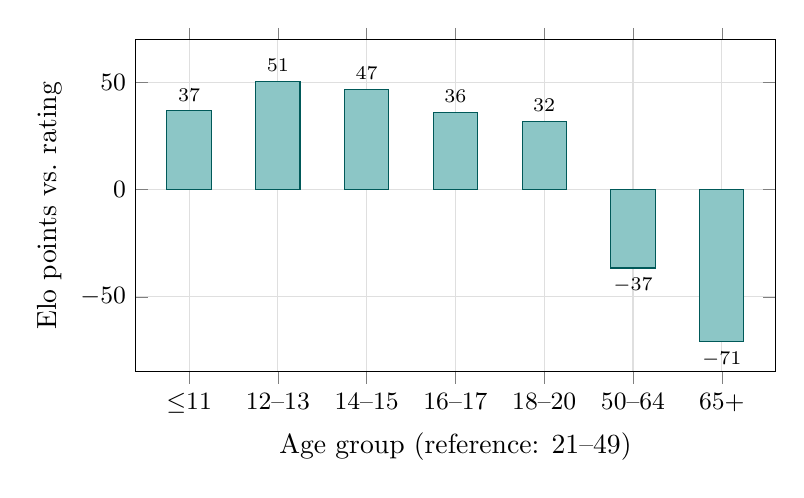
\begin{tikzpicture}
\begin{axis}[ybar, width=0.8\linewidth, height=5.8cm, bar width=16pt, ylabel={Elo points vs.\ rating}, xlabel={Age group (reference: 21--49)}, xtick={1,...,7}, xticklabels={$\leq$11,12--13,14--15,16--17,18--20,50--64,65+}, xmin=0.4, xmax=7.6, ymin=-85, ymax=70, grid=major, grid style={gray!25}, tick label style={font=\small}, nodes near coords, nodes near coords style={font=\scriptsize}, every node near coord/.append style={/pgf/number format/fixed, /pgf/number format/precision=0}]
\addplot[fill=teal!45, draw=teal!70!black] coordinates {(1,36.8) (2,50.7) (3,46.7) (4,36.2) (5,31.8) (6,-36.5) (7,-71.0)};
\end{axis}
\end{tikzpicture}

\caption{Fitted age offsets in Elo points relative to players aged 21 to 49, training season 2024--25 (model with white advantage and age groups).}
\label{fig:age}
\end{figure}

\subsection{Players returning from a break}

Figure~\ref{fig:decay} shows score against FIDE's expectation by the length of the player's most recent break, pooled over all test seasons. For adults the gap widens steadily with the length of the break and is larger for older players. Returning juniors show the opposite pattern: they outperform their ratings, as they did when active.

Table~\ref{tab:inactivity} gives the fitted offsets. For adults aged 21 to 49 the offset is \DecayMidOneTwo{} points after a break of one to two years, \DecayMidTwoFour{} after two to four years and \DecayMidFour{} after four years or more; for players over 50 it is \DecayOldOneTwo{}, \DecayOldTwoFour{} and \DecayOldFour{}. For juniors returning after one to two years it is \DecayYoungOneTwo{}. The offsets in the first column are measured against the average active player, so for older players they include the general age effect; the second column controls for age group and recent form (Section~\ref{sec:robust}).

\begin{figure}[htbp]
\centering
\begin{tikzpicture}
\begin{axis}[width=0.8\linewidth, height=6.2cm, xlabel={Time since last rated classical game}, ylabel={Score vs.\ expectation (points per 100 games)},
  xtick={0,1,2,3,4,5}, xticklabels={Active,3--5 mo,6--11 mo,1--2 yr,2--4 yr,4+ yr}, ymin=-20, ymax=6, grid=major, grid style={gray!25},
  legend pos=south west, legend style={font=\small, draw=none}, tick label style={font=\small}]
\addplot[thick, mark=*, color=teal!70!black] table {generated/plot_decay_young.dat};
\addplot[thick, mark=square*, color=brown!80!black] table {generated/plot_decay_mid.dat};
\addplot[thick, mark=triangle*, color=red!60!black] table {generated/plot_decay_old.dat};
\legend{Under 21, 21--49, 50 and over}
\end{axis}
\end{tikzpicture}
\caption{Score against FIDE's expectation by time since the player's last rated classical game, all eleven test seasons pooled. Groups with fewer than 150 player-games are not drawn.}
\label{fig:decay}
\end{figure}

\begin{table}[htbp]
\centering
\small
\caption{Fitted rating offsets for players returning from a break, in Elo points, all seasons. \emph{Plain}: offsets relative to the average active player. \emph{Controlled}: also controlling for age group and recent form.}
\label{tab:inactivity}
\begin{tabular}{llrrr}
\toprule
Age group & Break & Player-games & Plain & Controlled \\
\midrule
\tabinput{generated/table_inactivity.tex}
\bottomrule
\end{tabular}
\end{table}

\subsection{Recent form and colour}

Recent form predicts results beyond the rating: a player running a tenth of a point per game above expectation plays about \FormTenth{} points above their rating in the following games. This is the signature of a rating that updates too slowly. The first move is worth about \WhiteElo{} rating points, and the fitted value stayed between \WhiteMin{} and \WhiteMax{} in every season. FIDE ignores colour in its expected score, which is reasonable for the rating list because colours balance over an event, but it is the simplest correction available for forecasting single games.

\subsection{Walk-forward results}

Table~\ref{tab:backtest} pools the eleven test seasons. Each correction beat the published ratings in every test season, and together they reduce the Brier score from \BrierFide{} to \BrierFull{}, a reduction of \WFGain{}. Table~\ref{tab:seasons} and Figure~\ref{fig:seasons} show the gains by season. They grew through the pandemic seasons, peaked in 2022--23 and fell after FIDE's March 2024 adjustment, but never came close to zero.

The last two rows of Table~\ref{tab:backtest} rebuild ratings from scratch, using only the games in this sample, under FIDE's Elo rule and under Glicko-2 \citep{glickman2001}. Both do far worse than the published list, which draws on every rated game in the world. Compared with each other on identical data, neither is consistently better: Glicko-2 had the lower log loss in \GlickoWins{} of \NSeasons{} seasons.

\begin{table}[htbp]
\centering
\small
\caption{Pooled walk-forward results over \NTestGames{} test games in \NSeasons{} test seasons. Change is the difference in log loss against the published ratings, with a 95\% event-bootstrap interval. The last column counts test seasons with lower log loss than the published ratings.}
\label{tab:backtest}
\begin{tabular}{lrrlr}
\toprule
Model & Log loss & Brier & Change in log loss & Better \\
\midrule
\tabinput{generated/table_backtest.tex}
\bottomrule
\end{tabular}
\end{table}

\begin{table}[htbp]
\centering
\small
\caption{Results by season. \emph{Less error}: reduction in Brier score from all corrections combined, tested on that season. The last three columns are parameters fitted on that season: gap scale $\gamma$, offset for ages 12 to 13, and white advantage, in Elo points.}
\label{tab:seasons}
\begin{tabular}{lrrrrr}
\toprule
Season & Games & Less error & Gap scale & Ages 12--13 & White \\
\midrule
\tabinput{generated/table_seasons.tex}
\bottomrule
\end{tabular}
\end{table}

\begin{figure}[htbp]
\centering
\begin{tikzpicture}
\begin{axis}[width=0.8\linewidth, height=6cm, xlabel={Test season (starting year)}, ylabel={Reduction in Brier score (\%)},
  ymin=0, grid=major, grid style={gray!25}, legend pos=north west, legend style={font=\small, draw=none},
  xtick={2015,2017,2019,2021,2023,2025}, x tick label style={/pgf/number format/1000 sep={}}, tick label style={font=\small}]
\addplot[thick, mark=*, color=black] table {generated/plot_seasons_full.dat};
\addplot[thick, mark=square*, color=teal!70!black] table {generated/plot_seasons_age.dat};
\addplot[thick, mark=triangle*, color=brown!80!black] table {generated/plot_seasons_gap.dat};
\addplot[thick, dashed, color=gray] table {generated/plot_seasons_white.dat};
\legend{All corrections, Age, Gap scale, White advantage}
\end{axis}
\end{tikzpicture}
\caption{Reduction in Brier score against the published ratings by test season. Each correction was fitted on the season before.}
\label{fig:seasons}
\end{figure}

\subsection{Replaying the rules}

Table~\ref{tab:sim} gives the replay results. The stretched table and the inactivity adjustment each beat FIDE's current rules in all eleven test seasons, and together they reduce the Brier score by \SimGain{}. The inactivity adjustment applied \ReturnsAdjusted{} times over the eleven seasons.

Both changes to the K-factor made forecasts worse in every season. A larger K for juniors mostly amplifies the noise in their results rather than tracking their improvement. The uncertainty-based K-factor, which raises K after a break so that a returning player's rating moves faster, did the same, and when combined with the other two rules it removed much of their gain. For returning players, a one-time adjustment works better than a faster-moving rating.

\begin{table}[htbp]
\centering
\small
\caption{Month-by-month replay of rule changes, pooled over \NSeasons{} test seasons. Change is the difference in log loss against FIDE's current rules, with a 95\% event-bootstrap interval.}
\label{tab:sim}
\begin{tabular}{lrrlr}
\toprule
Rule set & Log loss & Brier & Change in log loss & Better \\
\midrule
\tabinput{generated/table_simulation.tex}
\bottomrule
\end{tabular}
\end{table}

\subsection{Inactivity at the top of the list}

Table~\ref{tab:top} lists the players rated 2700 or above on the September 2026 list who are flagged inactive, and one active player for contrast. FIDE keeps their ratings unchanged. The last column shows the adjustment the fitted inactivity rule would apply if they returned. These are averages estimated mostly from non-elite players and are shown only to illustrate the rule's scale.

\begin{table}[htbp]
\centering
\small
\caption{Players rated 2700 or above on the September 2026 FIDE list who are flagged inactive, and one active player for contrast. Games are rated classical games in the last 12 lists.}
\label{tab:top}
\begin{tabular}{lrrlrrr}
\toprule
Player & Rating & Age & Status & Games & Months since last & Return adjustment \\
\midrule
\tabinput{generated/table_top.tex}
\bottomrule
\end{tabular}
\end{table}

\section{Robustness}
\label{sec:robust}

\paragraph{Is the inactivity effect just age or prior decline?} Players who stop playing may already have been declining. Refitting the inactivity offsets while also controlling for age group and each player's recent form before the game (Table~\ref{tab:inactivity}, last column) shrinks the offsets, most of all for older players, whose general overrating is now absorbed by the age terms. A clear effect remains: \DecayMidFourCtrl{} points for adults aged 21 to 49 after four years or more, \DecayOldFourCtrl{} for players over 50, and \DecayYoungOneTwoCtrl{} for juniors returning after one to two years. The size of the effect still grows with the length of the break in every age group.

\paragraph{Does the gap scale depend on rating level?} Table~\ref{tab:gapband} fits the gap scale separately by the higher-rated player's rating. The scale is below 1 in every band, but it depends strongly on rating: \GapBandLow{} when the higher-rated player is below 1800 and \GapBandTop{} when they are rated 2500 or above. The table is therefore close to right at the top of the list and much too steep lower down. The white advantage also grows with rating level.

\begin{table}[htbp]
\centering
\small
\caption{Gap scale fitted separately by the higher-rated player's rating, all test seasons.}
\label{tab:gapband}
\begin{tabular}{lrrr}
\toprule
Higher-rated player & Games & Gap scale & White (Elo) \\
\midrule
\tabinput{generated/table_gapband.tex}
\bottomrule
\end{tabular}
\end{table}

\paragraph{Is the inactivity effect the same for stronger players?} Table~\ref{tab:level} splits the adult inactivity pattern by rating. The decline with break length appears at every rating level, including players rated 2300 and above.

\begin{table}[htbp]
\centering
\small
\caption{Adults (21 and over): score against FIDE's expectation (points per 100 games) by break length and rating, all test seasons. Player-games in brackets.}
\label{tab:level}
\begin{tabular}{llll}
\toprule
Break & Below 2000 & 2000--2299 & 2300+ \\
\midrule
\tabinput{generated/table_level.tex}
\bottomrule
\end{tabular}
\end{table}

\paragraph{Did the pandemic drive the results?} Leaving out the 2019--20 and 2020--21 seasons, the combined corrections still change log loss by \NoPandemicFull{} against the published ratings (pooled: \FullLogLoss{}), and the replayed table-plus-inactivity rule by \NoPandemicSim{} against FIDE's rules (pooled: \SimLogLoss{}).

\section{Discussion}

The published FIDE ratings carry four systematic errors, and all four held in every test season. Two of them translate directly into rule changes that FIDE could adopt: widening the expectancy table and adjusting the ratings of returning players by age and length of break. Both improved forecasts in every season when replayed against the actual K-factors FIDE used.

The table result comes with a qualification. The gap scale is close to 1 among players rated 2500 and above and far below 1 lower down, so a single wider table would fix most of the error for the bulk of the list while slightly understating gaps at the top. Part of the low-rating effect may reflect juniors, who are both lower-rated and underrated. A table whose width depends on rating level, or a direct fix for junior ratings, may do better than one uniform table; both are worth testing.

The inactivity result bears on a long-standing debate about rating decay. FIDE keeps an inactive player's rating unchanged indefinitely. The evidence here supports a decay for adults, larger with age and with the length of the break, but not a flat decay for everyone: juniors who return are, if anything, underrated. A one-time adjustment on return did better than an uncertainty-based K-factor that lets the rating move faster afterwards, which suggests that returning players' ratings are biased, not merely noisy.

The junior problem remains open. Juniors are underrated in every season, but neither a larger K-factor nor an uncertainty-based K-factor helped. A rule that expects improvement by age, for example an age-dependent drift term in the rating update, is a natural next test.

\paragraph{Limitations.} The sample leans toward stronger and better-documented events; club-level play needs separate data. The replay updates ratings only from games in the sample, so a rule adopted by FIDE would act on more games than the replay sees. Birth years come from the current player list, and breaks are measured to the nearest month. The 400-point rule is applied to all players, although since October 2025 it no longer applies to players rated 2650 or above; this affects very few games. Finally, the inactivity offsets are averages, and individual returning players may differ widely from them.

\section{Conclusion}

Twelve seasons of classical games show that the FIDE rating list misprices rating gaps, age and inactivity in consistent ways. A wider expectancy table and an age-dependent adjustment for returning players would have beaten the current rules in every one of eleven test seasons. Changes to the K-factor would not have.

\section*{Data and code availability}

All code is available at \url{https://github.com/nipuncanyou/fide-rating-research}, and an interactive report at \url{https://nipuncanyou.github.io/fide-rating-research/report/}. Game data is from The Week in Chess and rating data from FIDE's public download page; the repository contains scripts that download both and reproduce every table and figure.

\bibliographystyle{plainnat}
\bibliography{references}

\end{document}
